\documentclass{article}
\usepackage{graphicx}
\usepackage{geometry}
\usepackage{hyperref}
\usepackage{subcaption}
\usepackage{amsmath}

\geometry{a4paper, margin=0.65in}

\hypersetup{
    colorlinks=true,
    linkcolor=blue,
    filecolor=magenta,      
    urlcolor=cyan,
}

\title{Spiking Threshold Sweep Comparison Report:\\$\theta \in \{1.0, 0.8, 0.6, 0.4\}$ on MNIST SNN}
\author{ByzFL SNN Benchmark}
\date{\today}

\begin{document}

\maketitle

\clearpage
\tableofcontents
\clearpage

\section{Introduction}
This report compiles and compares the robust aggregation sweep results for different values of the spiking threshold $\theta \in \{1.0, 0.8, 0.6, 0.4\}$. All models are SNNs trained with constant encoding ($T=10$) and the Atan surrogate gradient ($\alpha = 1.2$).
We compare the worst-case test accuracy across four robust aggregators (Centered Clipping, Geometric Median, Multi-Krum, and Trimmed Mean) under three different attacks:
\begin{enumerate}
    \item Optimal A Little Is Enough (OptALIE)
    \item Optimal Inner Product Manipulation (OptIPM)
    \item Sign Flipping
\end{enumerate}
Our objective is to verify whether varying the spiking threshold alters the gradient sparsity and consequently shifts the vulnerability window of the SNN.

\clearpage
\section{Worst-Case Robustness (Across All Attacks)}
The following figures show the worst-case test accuracy across all three attacks for the different threshold values.

\begin{figure}[htbp]
    \centering
    \begin{subfigure}[b]{0.48\textwidth}
        \centering
        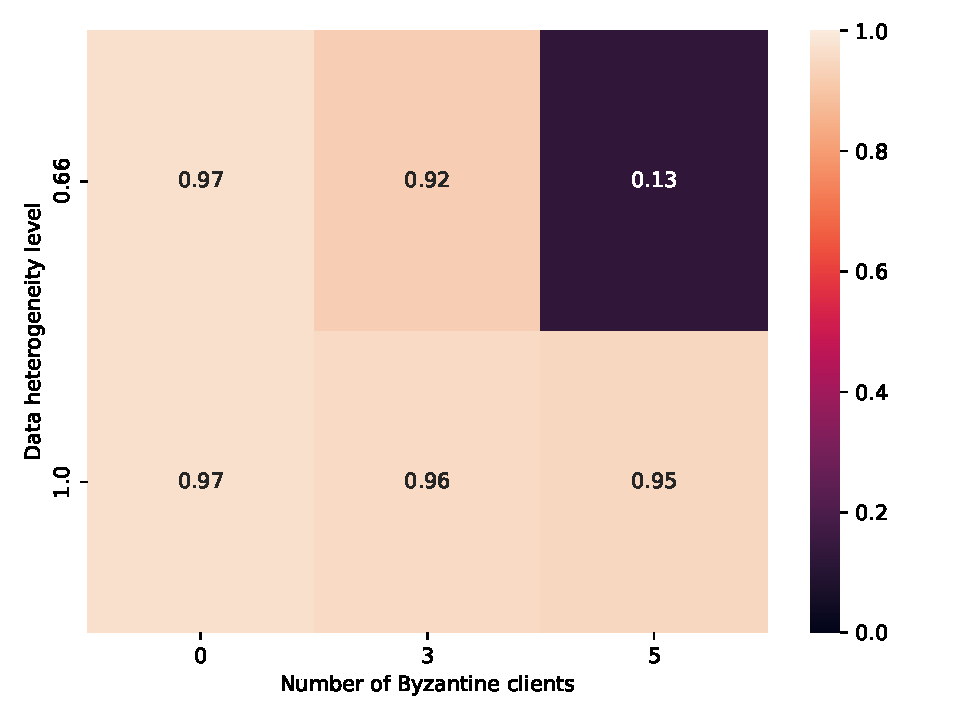
\includegraphics[width=\textwidth]{../plots/threshold_sweep/10/plots/best_test_mnist_cnn_mnist_snn_gamma_similarity_niid_NNM_ARC_nb_honest_clients_10_tolerated_f_equal_real.pdf}
        \caption{$\theta = 1.0$}
    \end{subfigure}
    \hfill
    \begin{subfigure}[b]{0.48\textwidth}
        \centering
        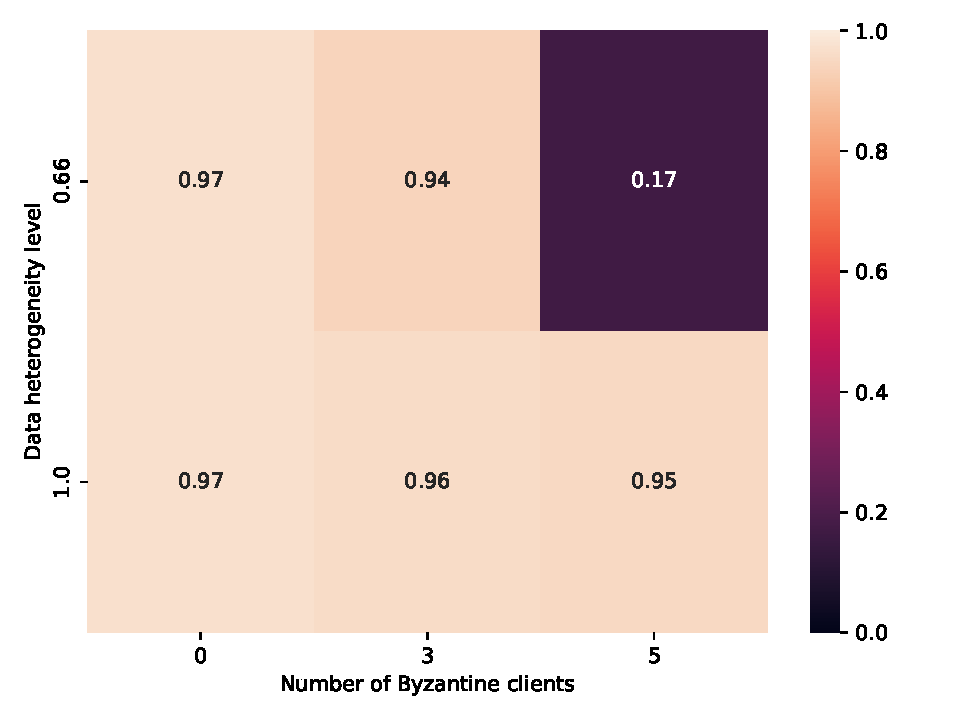
\includegraphics[width=\textwidth]{../plots/threshold_sweep/08/plots/best_test_mnist_cnn_mnist_snn_gamma_similarity_niid_NNM_ARC_nb_honest_clients_10_tolerated_f_equal_real.pdf}
        \caption{$\theta = 0.8$}
    \end{subfigure}
    \vspace{0.3cm}
    \begin{subfigure}[b]{0.48\textwidth}
        \centering
        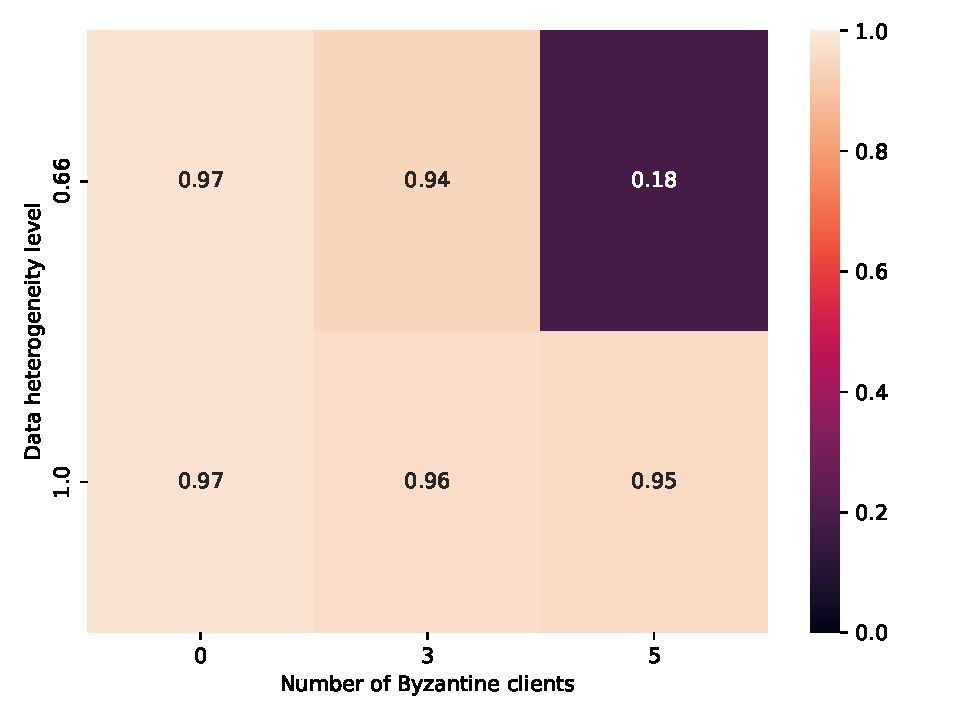
\includegraphics[width=\textwidth]{../plots/threshold_sweep/06/plots/best_test_mnist_cnn_mnist_snn_gamma_similarity_niid_NNM_ARC_nb_honest_clients_10_tolerated_f_equal_real.pdf}
        \caption{$\theta = 0.6$}
    \end{subfigure}
    \hfill
    \begin{subfigure}[b]{0.48\textwidth}
        \centering
        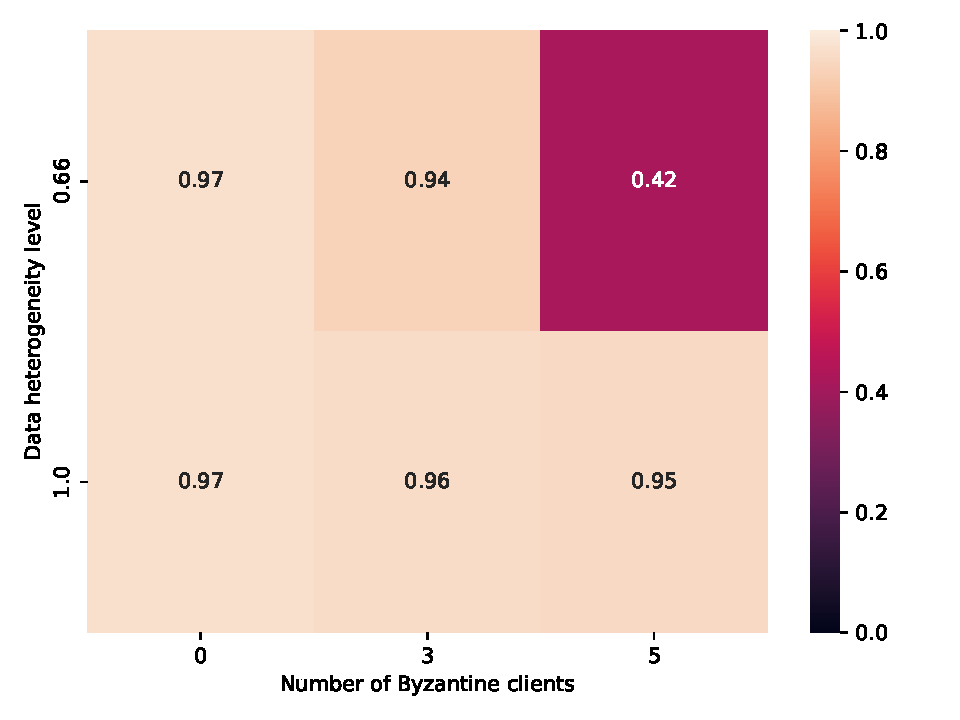
\includegraphics[width=\textwidth]{../plots/threshold_sweep/04/plots/best_test_mnist_cnn_mnist_snn_gamma_similarity_niid_NNM_ARC_nb_honest_clients_10_tolerated_f_equal_real.pdf}
        \caption{$\theta = 0.4$}
    \end{subfigure}
    \caption{Worst-case test accuracy across all attacks (Worst-Case Heatmaps) for different spiking thresholds.}
    \label{fig:worst_case_grid}
\end{figure}\clearpage
\section{Robustness under Optimal ALIE}\begin{figure}[htbp]
    \centering
    \begin{subfigure}[b]{0.48\textwidth}
        \centering
        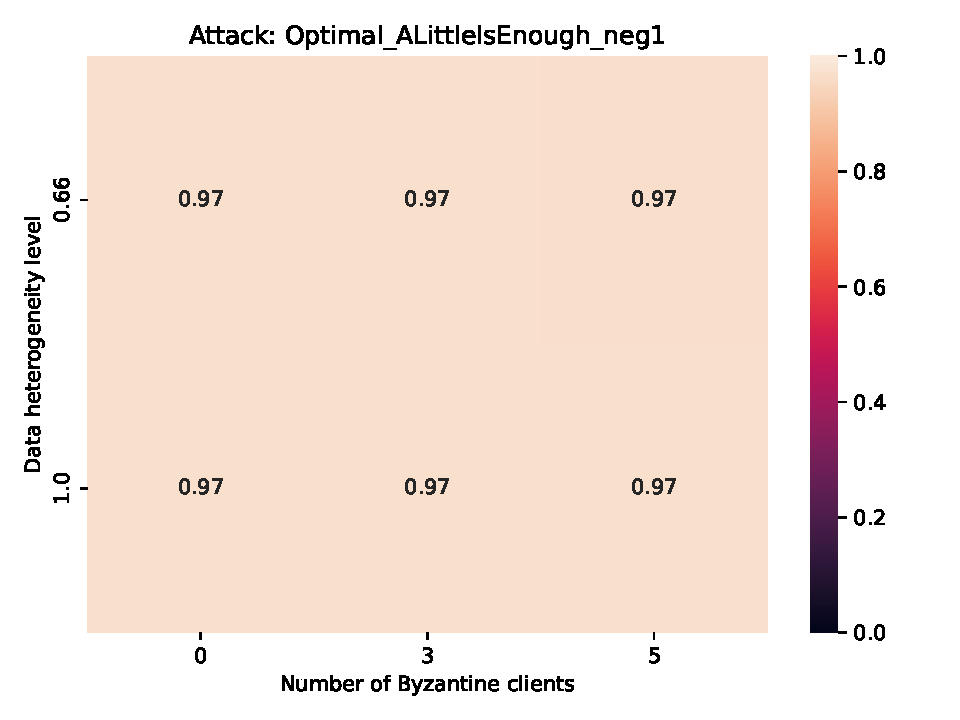
\includegraphics[width=\textwidth]{../plots/threshold_sweep/10/plots/best_test_Optimal_ALittleIsEnough_neg1_mnist_cnn_mnist_snn_gamma_similarity_niid_NNM_ARC_nb_honest_clients_10_tolerated_f_equal_real.pdf}
        \caption{$\theta = 1.0$}
    \end{subfigure}
    \hfill
    \begin{subfigure}[b]{0.48\textwidth}
        \centering
        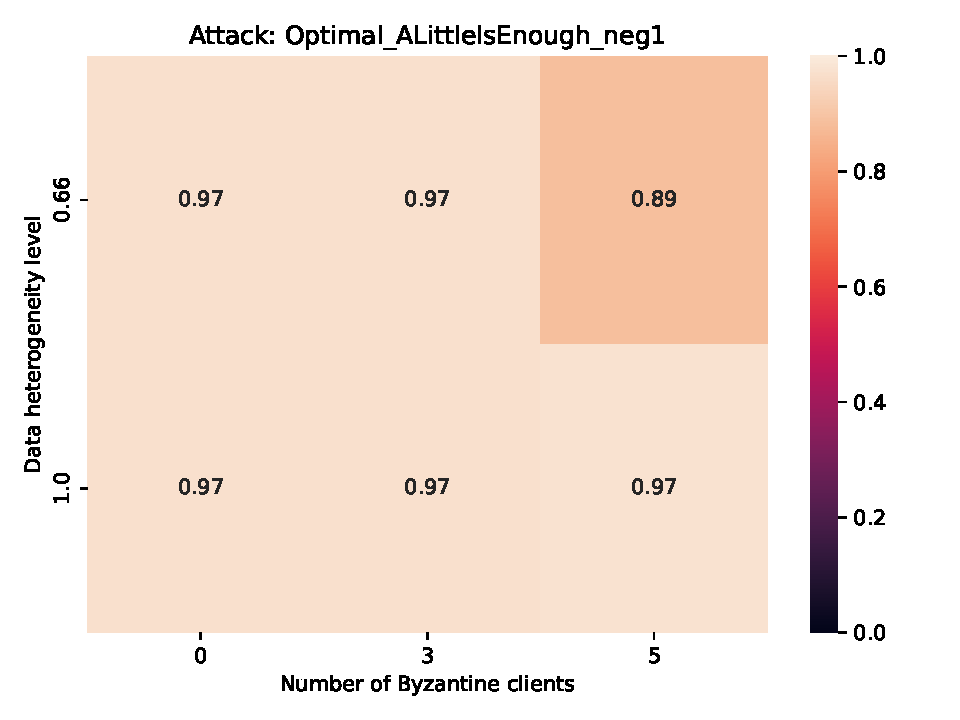
\includegraphics[width=\textwidth]{../plots/threshold_sweep/08/plots/best_test_Optimal_ALittleIsEnough_neg1_mnist_cnn_mnist_snn_gamma_similarity_niid_NNM_ARC_nb_honest_clients_10_tolerated_f_equal_real.pdf}
        \caption{$\theta = 0.8$}
    \end{subfigure}
    \vspace{0.3cm}
    \begin{subfigure}[b]{0.48\textwidth}
        \centering
        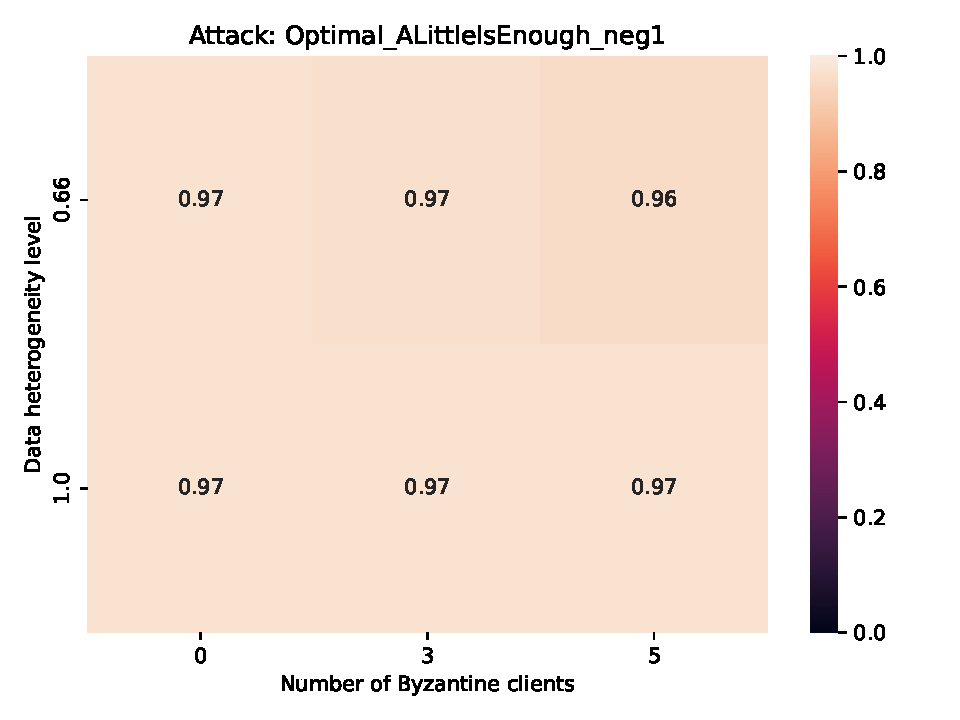
\includegraphics[width=\textwidth]{../plots/threshold_sweep/06/plots/best_test_Optimal_ALittleIsEnough_neg1_mnist_cnn_mnist_snn_gamma_similarity_niid_NNM_ARC_nb_honest_clients_10_tolerated_f_equal_real.pdf}
        \caption{$\theta = 0.6$}
    \end{subfigure}
    \hfill
    \begin{subfigure}[b]{0.48\textwidth}
        \centering
        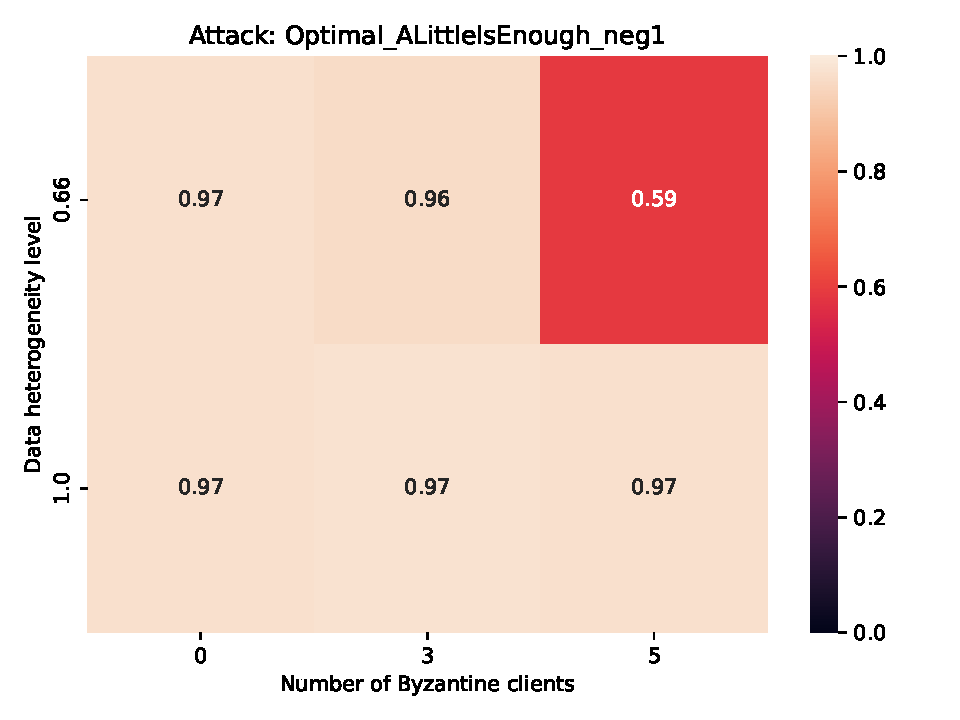
\includegraphics[width=\textwidth]{../plots/threshold_sweep/04/plots/best_test_Optimal_ALittleIsEnough_neg1_mnist_cnn_mnist_snn_gamma_similarity_niid_NNM_ARC_nb_honest_clients_10_tolerated_f_equal_real.pdf}
        \caption{$\theta = 0.4$}
    \end{subfigure}
    \caption{Test accuracy under Optimal A Little Is Enough (OptALIE) attack for different spiking thresholds.}
    \label{fig:opt_alie_grid}
\end{figure}\clearpage
\section{Robustness under Optimal IPM}\begin{figure}[htbp]
    \centering
    \begin{subfigure}[b]{0.48\textwidth}
        \centering
        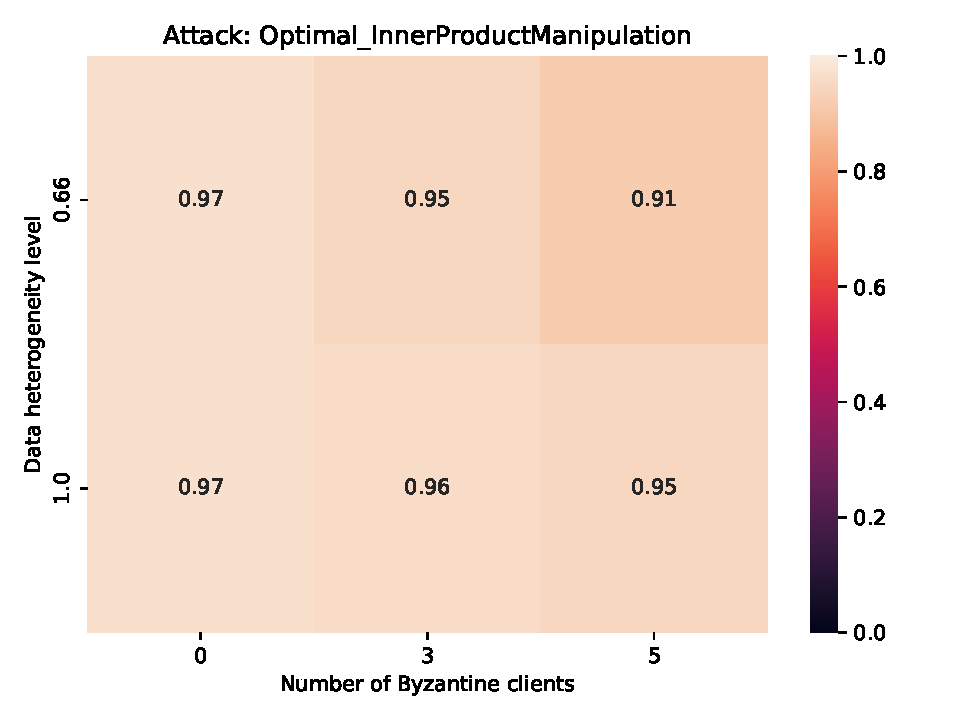
\includegraphics[width=\textwidth]{../plots/threshold_sweep/10/plots/best_test_Optimal_InnerProductManipulation_mnist_cnn_mnist_snn_gamma_similarity_niid_NNM_ARC_nb_honest_clients_10_tolerated_f_equal_real.pdf}
        \caption{$\theta = 1.0$}
    \end{subfigure}
    \hfill
    \begin{subfigure}[b]{0.48\textwidth}
        \centering
        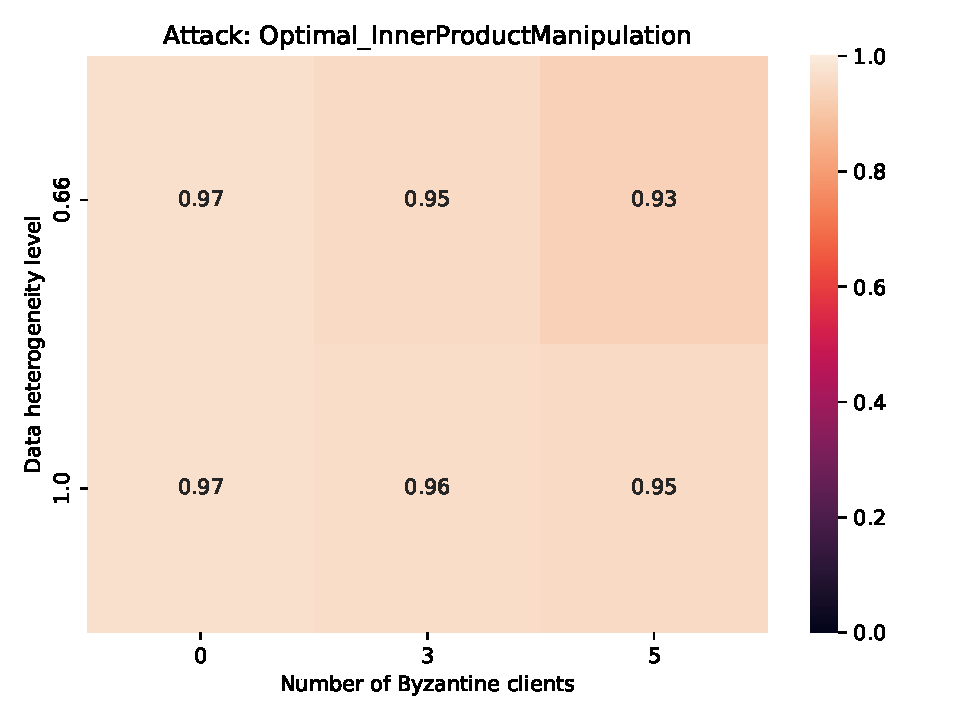
\includegraphics[width=\textwidth]{../plots/threshold_sweep/08/plots/best_test_Optimal_InnerProductManipulation_mnist_cnn_mnist_snn_gamma_similarity_niid_NNM_ARC_nb_honest_clients_10_tolerated_f_equal_real.pdf}
        \caption{$\theta = 0.8$}
    \end{subfigure}
    \vspace{0.3cm}
    \begin{subfigure}[b]{0.48\textwidth}
        \centering
        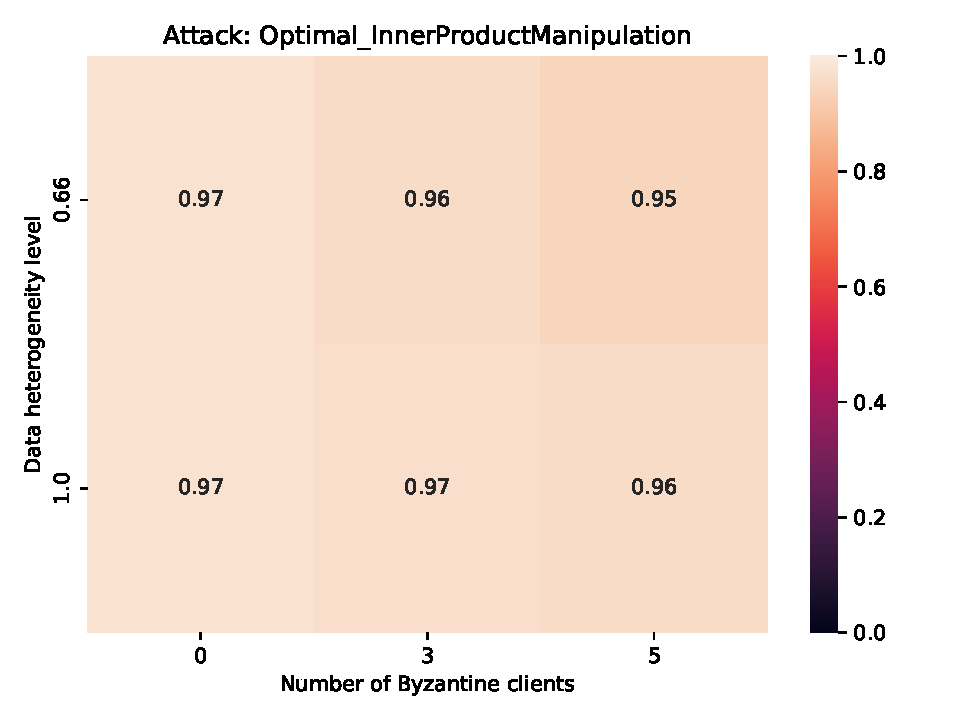
\includegraphics[width=\textwidth]{../plots/threshold_sweep/06/plots/best_test_Optimal_InnerProductManipulation_mnist_cnn_mnist_snn_gamma_similarity_niid_NNM_ARC_nb_honest_clients_10_tolerated_f_equal_real.pdf}
        \caption{$\theta = 0.6$}
    \end{subfigure}
    \hfill
    \begin{subfigure}[b]{0.48\textwidth}
        \centering
        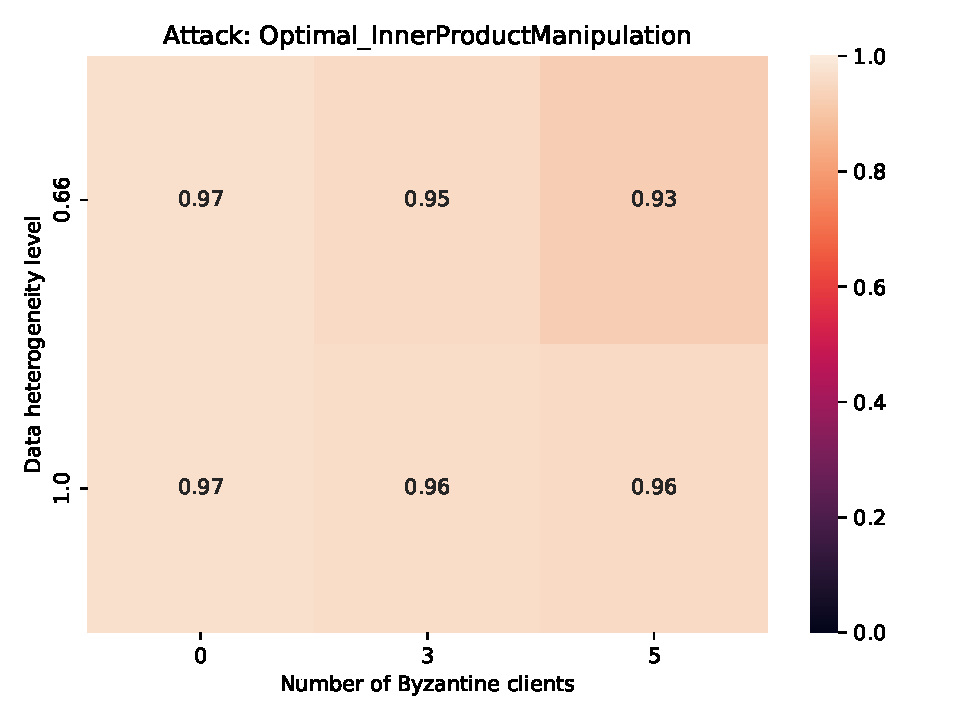
\includegraphics[width=\textwidth]{../plots/threshold_sweep/04/plots/best_test_Optimal_InnerProductManipulation_mnist_cnn_mnist_snn_gamma_similarity_niid_NNM_ARC_nb_honest_clients_10_tolerated_f_equal_real.pdf}
        \caption{$\theta = 0.4$}
    \end{subfigure}
    \caption{Test accuracy under Optimal Inner Product Manipulation (OptIPM) attack for different spiking thresholds.}
    \label{fig:opt_ipm_grid}
\end{figure}\clearpage
\section{Robustness under Sign Flipping}\begin{figure}[htbp]
    \centering
    \begin{subfigure}[b]{0.48\textwidth}
        \centering
        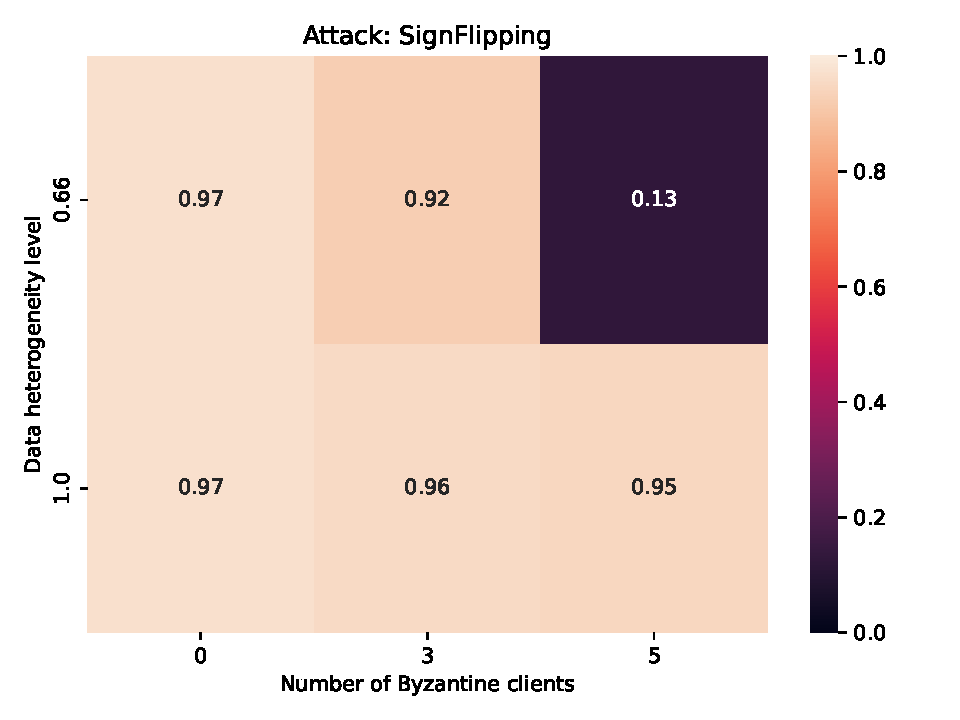
\includegraphics[width=\textwidth]{../plots/threshold_sweep/10/plots/best_test_SignFlipping_mnist_cnn_mnist_snn_gamma_similarity_niid_NNM_ARC_nb_honest_clients_10_tolerated_f_equal_real.pdf}
        \caption{$\theta = 1.0$}
    \end{subfigure}
    \hfill
    \begin{subfigure}[b]{0.48\textwidth}
        \centering
        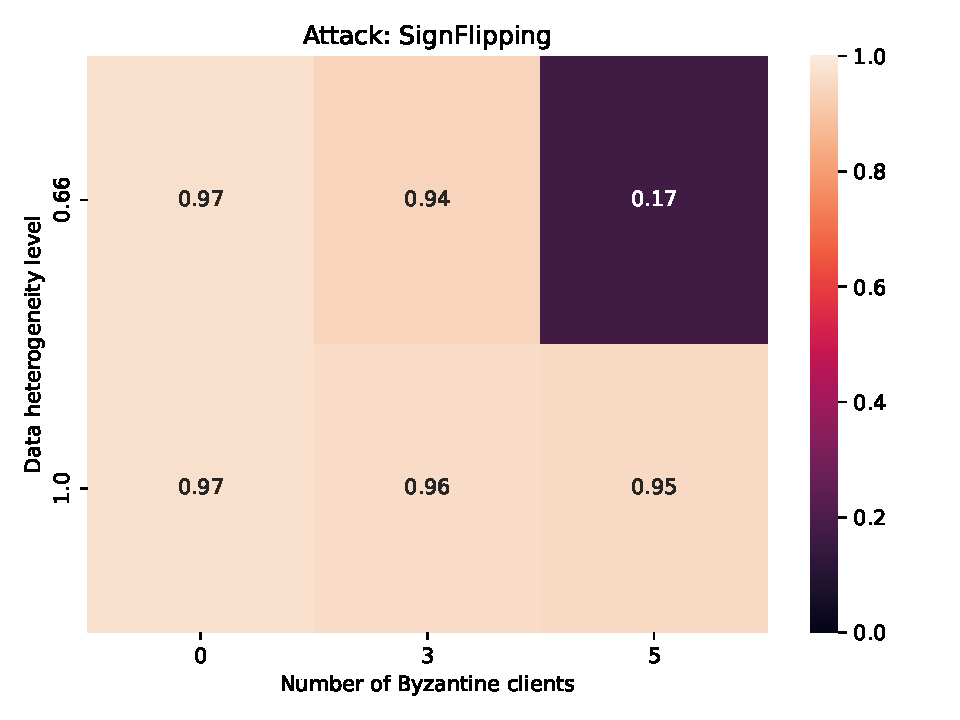
\includegraphics[width=\textwidth]{../plots/threshold_sweep/08/plots/best_test_SignFlipping_mnist_cnn_mnist_snn_gamma_similarity_niid_NNM_ARC_nb_honest_clients_10_tolerated_f_equal_real.pdf}
        \caption{$\theta = 0.8$}
    \end{subfigure}
    \vspace{0.3cm}
    \begin{subfigure}[b]{0.48\textwidth}
        \centering
        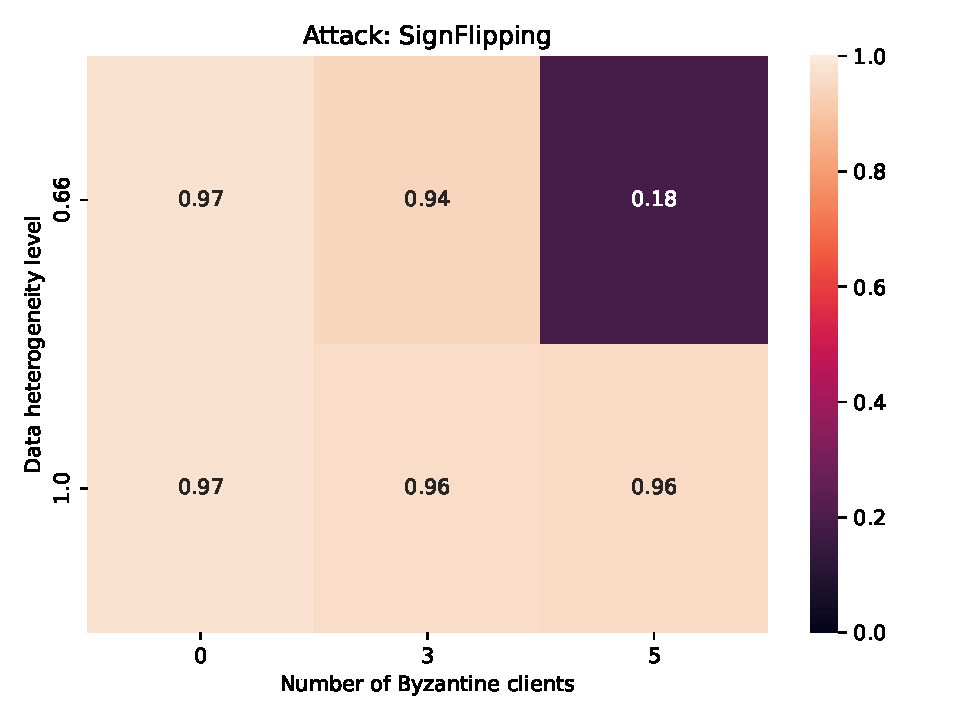
\includegraphics[width=\textwidth]{../plots/threshold_sweep/06/plots/best_test_SignFlipping_mnist_cnn_mnist_snn_gamma_similarity_niid_NNM_ARC_nb_honest_clients_10_tolerated_f_equal_real.pdf}
        \caption{$\theta = 0.6$}
    \end{subfigure}
    \hfill
    \begin{subfigure}[b]{0.48\textwidth}
        \centering
        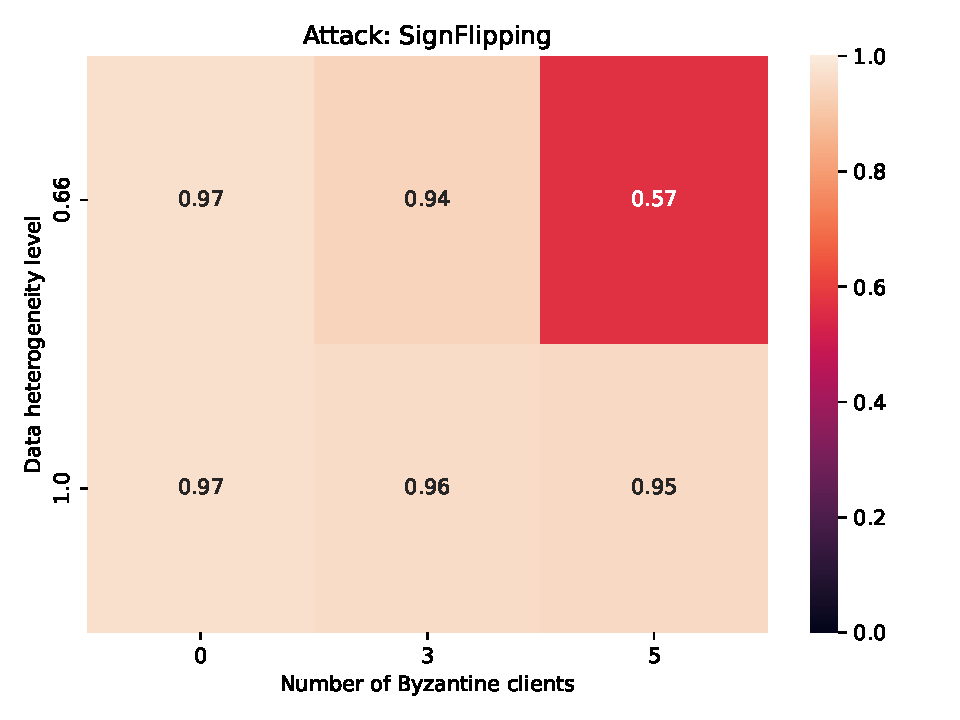
\includegraphics[width=\textwidth]{../plots/threshold_sweep/04/plots/best_test_SignFlipping_mnist_cnn_mnist_snn_gamma_similarity_niid_NNM_ARC_nb_honest_clients_10_tolerated_f_equal_real.pdf}
        \caption{$\theta = 0.4$}
    \end{subfigure}
    \caption{Test accuracy under Sign Flipping attack for different spiking thresholds.}
    \label{fig:sign_flipping_grid}
\end{figure}\clearpage

\end{document}
